\documentclass{article}

\usepackage[spanish]{babel}
\usepackage{listings}
\usepackage{color}
\usepackage[numbers,sort&compress]{natbib}
\usepackage{graphicx}
\usepackage{subfigure}
\usepackage{url}
\usepackage{amsmath}
\usepackage{hyperref}
\usepackage[top=15mm, bottom=40mm, left=15mm, right=15mm]{geometry}
\setlength{\parskip}{2mm}
\setlength{\parindent}{0pt}

\setlength{\parskip}{2mm}
\setlength{\parindent}{0pt}
\definecolor{blue}{rgb}{0,0.6,0}
\definecolor{gray}{rgb}{0.3,0.3,0.3}
\definecolor{orange}{rgb}{0.8,0.4,0}
\definecolor{mostaza}{rgb}{0.9,0.8,0.1}

\lstset{ %
  language=R,                     % the language of the code
  basicstyle=\footnotesize,       % the size of the fonts that are used for the code
  numbers=left,                   % where to put the line-numbers
  numberstyle=\tiny\color{gray},  % the style that is used for the line-numbers
  stepnumber=1,                   % the step between two line-numbers. If it's 1, each line
                                  % will be numbered
  numbersep=5pt,                  % how far the line-numbers are from the code
  backgroundcolor=\color{white},  % choose the background color. You must add \usepackage{color}
  showspaces=false,               % show spaces adding particular underscores
  showstringspaces=false,         % underline spaces within strings
  showtabs=false,                 % show tabs within strings adding particular underscores
  frame=single,                   % adds a frame around the code
  rulecolor=\color{black},        % if not set, the frame-color may be changed on line-breaks within not-black text (e.g. commens (green here))
  tabsize=2,                      % sets default tabsize to 2 spaces
  captionpos=b,                   % sets the caption-position to bottom
  breaklines=true,                % sets automatic line breaking
  breakatwhitespace=false,        % sets if automatic breaks should only happen at whitespace
  title=\lstname,                 % show the filename of files included with \lstinputlisting;
                                  % also try caption instead of title
  keywordstyle=\color{orange},      % keyword style
  commentstyle=\color{blue},   % comment style
  stringstyle=\color{mostaza},      % string literal style
  escapeinside={\%*}{*)},         % if you want to add a comment within your code
  morekeywords={*,...}            % if you want to add more keywords to the set
} 

\author{1445183}
\title{Práctica 6: Sistema multiagente}
\date{\today}

\begin{document}

\maketitle

\section{Objetivo}
Encontrar el porcentaje máximo de agentes infectados previamente vacunados dentro del sistema multiagente propuesto en esta práctica \cite{elisaweb6}.

\section{Descripción}
El sistema multiagente está compuesto por 50 agentes, los cuales se pueden encontrar en uno de los siguientes estados: \textit{suceptible, recuperado  o infectado}, de manera aleatoria. Los agentes se ``vacunan'' con una probabilidad $P_{v}$ de 0 a 1 con 30 réplicas para cada probabilidad, lo cual afectará a la cantidad de agentes en estado \textit{infectado} finales. 

\begin{lstlisting}[language=R]
Pv <- seq(0,1,0.1) #probabilidad
for(pv in Pv){ #vacuna
  for(rep in 1:30){
    agentes <- data.frame(x = double(), y = double(), dx = double(), dy = double(), estado  = character(), amigo = NULL)
    for (i in 1:n) { 
      if(runif(1) < pv){ 
        e <- "R"
      } else if(runif(1) < pi){
        e <- "I"
      } else{
        e <- "S"
      }
\end{lstlisting}

\newpage


\section{Resultados}

En la figura \ref{p6} se puede observa el porcentaje máximo de infectados para cada valor de probabilidad mostrando un decrecimiento conforme la probabilidad aumenta. El cuadro \ref{pormax} muestra más a detalle el valor máximo de porcentaje de infectados para cada probabilidad.

\begin{figure}[!h]
\centering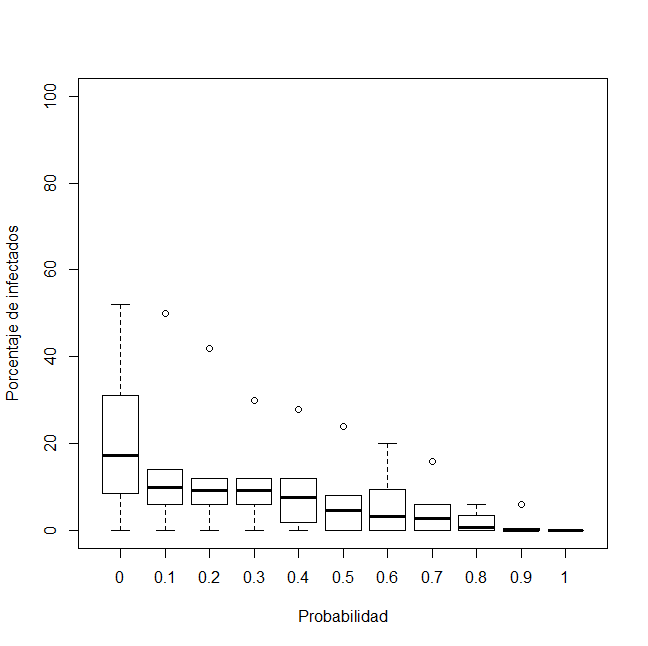
\includegraphics[width=100mm]{p6v2.png}
\caption{Porcentaje de infectados vs probabilidad}
\label{p6}
\end{figure}

\begin{table}[h!]
\caption{Valores de porcentajes máximos}
\label{pormax}
\vspace*{3mm}
\centering
\begin{tabular}{l|c} 
Probabilidad & Porcentaje máximo de infectados \\  \hline
0 & 52 \\
0.1 &  50 \\
0.2 & 42 \\
0.3 & 30 \\
0.4 & 28 \\
0.5 & 24 \\
0.6 & 20 \\
0.7 & 16 \\
0.8 & 6 \\
0.9 & 6 \\
0.10 & 0 \\
\end{tabular}
\end{table}

\newpage

\section{Conclusiones}

La cantidad de agentes \textit{infectados} disminuye conforme aumenta la dosis de la vacuna, es decir, al aumentar la probabilidad $P_{v}$ aumenta la cantidad de agentes en estado \textit{recuperado} por lo que disminuye la cantidad de agentes \textit{infectados}.

\bibliographystyle{plainnat}
\bibliography{bibliosimu}

\end{document}